\chapter{Méthodes bio-informatiques pour explorer les EVEs et inférer leurs domestications moléculaires}
{\hypersetup{linkcolor=GREYDARK}\minitoc}
\label{chap:annexe-methods}


Lorsqu'il s'agit d'inférer des évènements de transferts horizontaux de gènes (THG) d'un clade à un autre, deux types de méthodes bio-informatiques existent. La première  dite "paramétrique" se base sur des caractéristiques particulières des clades étudiés qui pourraient appuyer l'hypothèse d'un THG. En effet, diverses signatures génomiques sont exploitables comme le contenu en GC le long d'un scaffold qui devrait changer à l'endroit où l'élément s'est intégré récemment (\figurename{\ref{figure:HGT_methods}}-A) \citep{ravenhall_inferring_2015}, ou bien la couverture génomique qui devrait changer selon les entités génomiques étudiées (\figurename{\ref{figure:HGT_methods}}-B). D'autres méthodes récemment développées se basent plutôt sur des résultats d'alignements de séquences, comme par exemple l'Alien index (AI) \citep{rancurel_alienness_2017} qui est une méthode qui compare les scores d'alignements de séquences provenant du groupe donneur (\figurename{\ref{figure:HGT_methods}}-C) (exemple : virus), avec les scores d'alignements du groupe receveur (exemple : insecte). Dans le cas où un gène viral a été effectivement transféré vers le génome d'une espèce d'insecte, alors le score d'alignement entre le locus d'insecte et les séquences de la base de données virale devrait être plus grand que l'alignement avec des séquences d’insectes. Un AI $>$ 0 indique une meilleure correspondance entre les taxons candidats donneurs et receveurs et un THG possible. Un AI plus élevé représente un écart plus important des scores d'alignements entre le candidat donneur et le receveur et un THG plus probable.

Enfin, un autre type de méthode se base plutôt sur la phylogénie (\figurename{\ref{figure:HGT_methods}}-D) \citep{ravenhall_inferring_2015}. Cette méthode est très efficace, car elle prend en compte l'histoire évolutive du transfert de gènes, c'est-à-dire la direction du transfert de gènes et les espèces d'où proviennent les gènes transférés. En inférant l'arbre des gènes et en le comparant à l'arbre des espèces de référence, les méthodes phylogénétiques identifient les incohérences dans l'histoire évolutive des gènes. Si un THG a été transféré d'un clade viral à un clade eucaryote, la phylogénie du gène viral devrait refléter une feuille eucaryote proche du taxon viral donneur (ou au moins un cousin) (\figurename{\ref{figure:HGT_methods}}-D). 

Quoi qu'il en soit, toutes ces méthodes ont leurs avantages et inconvénients et permettent de répondre à des problématiques particulières. Durant ma thèse, j'ai essayé d'adapter certains de ces méthodes paramétriques et phylogénétiques pour inférer des transferts de gènes de virus vers les génomes d'Hyménoptères.  

\begin{figure}[!htpb]
\captionsetup{font=footnotesize}
 \centering
  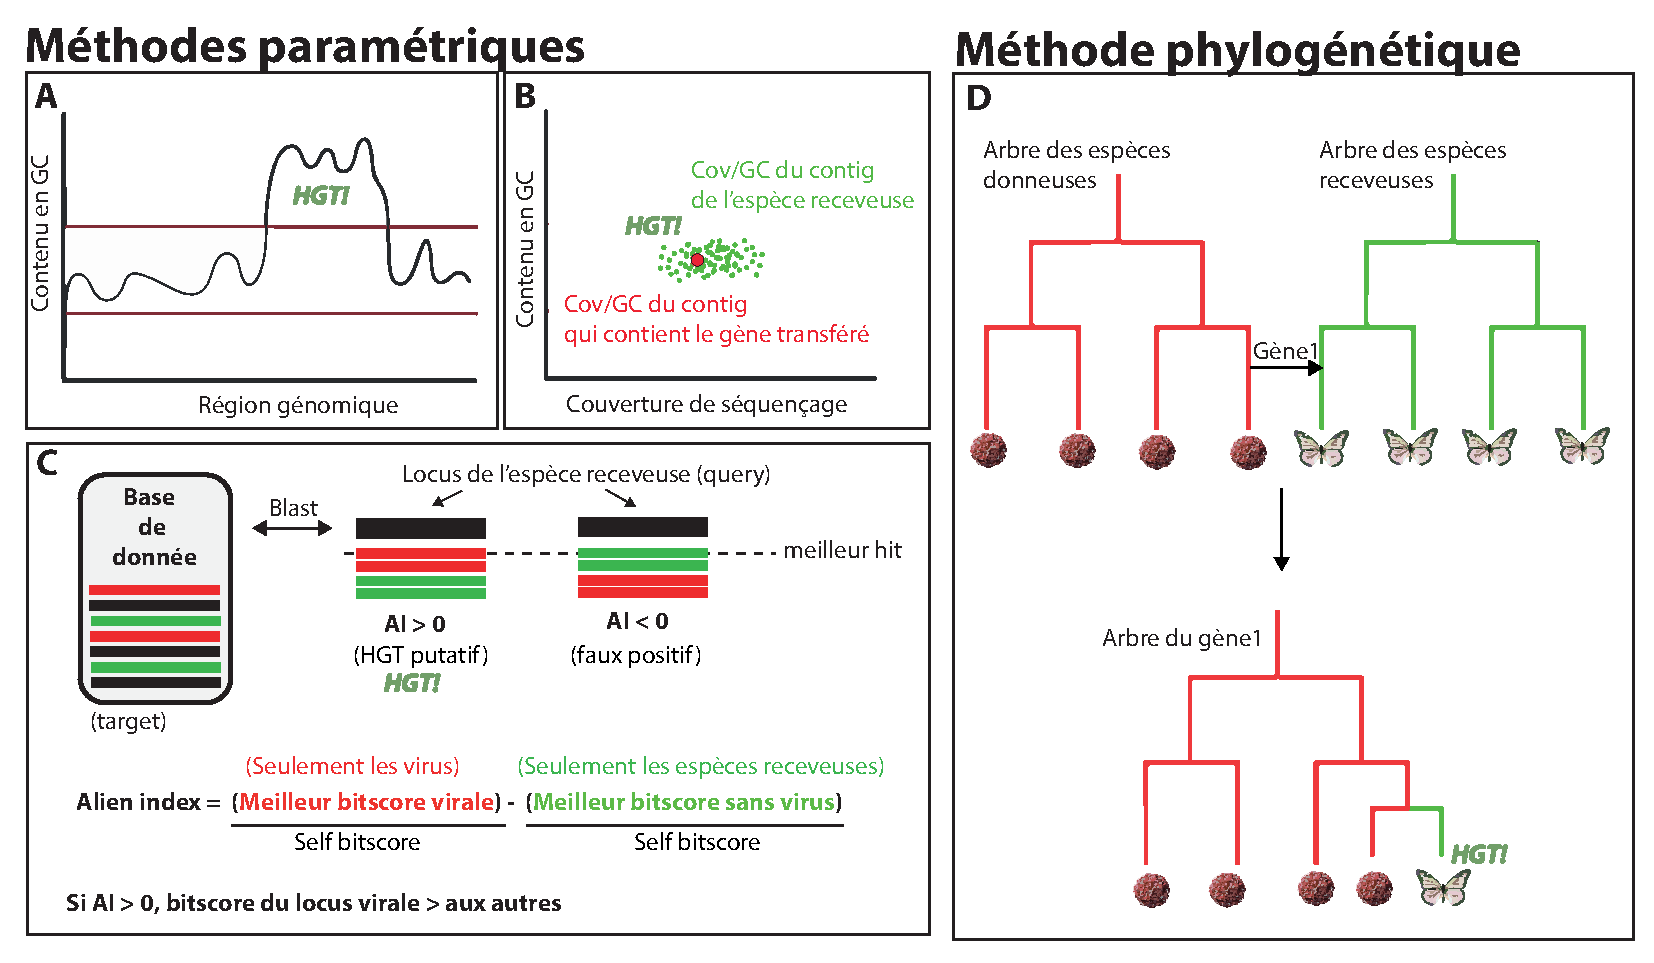
\includegraphics[width=\linewidth,height=\textheight,keepaspectratio]{PhD-master/figures/HGT_methods.pdf}
\caption[Methode:Aperçu conceptuel des méthodes d'inférence de transferts horizontaux]{\textbf{Aperçu conceptuel des méthodes d'inférence de transferts horizontaux inspiré de \cite{ravenhall_inferring_2015}}}
\label{figure:HGT_methods}
\end{figure}

Ces dernières années, plusieurs groupes de recherche ont tenté d'identifier l'endogénisation des séquences virales chez les arthropodes, et en particulier chez les Hyménoptères (tableau \ref{tab:Table_with_dEVEs_in_literature}). Une partie au moins de ces études a été motivée par les descriptions précédentes d'événements de domestication dans la superfamille des Ichneumonoidea.

% \usepackage{ragged2e}
% \usepackage{array}
% \usepackage{graphicx}
% \usepackage{booktabs}
% \usepackage{colortbl}


\begin{table}
\centering
\setlength{\extrarowheight}{0pt}
\addtolength{\extrarowheight}{\aboverulesep}
\addtolength{\extrarowheight}{\belowrulesep}
\setlength{\aboverulesep}{0pt}
\setlength{\belowrulesep}{0pt}
\caption[Methode:Criblages récents de virus dans les génomes d'arthropodes]{Criblages récents de virus dans les génomes d'arthropodes.}
\resizebox{\textwidth}{!}{\begin{tabular}{rlrrrlrr}
\toprule
\rowcolor[rgb]{0.8,0.8,0.8} \textbf{Article} & \textbf{Clades hôtes} & \textbf{Clades viraux} & \textbf{N génomes artrhopodes} & \textbf{Check évènements} & \textbf{Check contamination} & \textbf{\textit{dN/dS}}  & \textbf{RNAseq}\\ 
\hline
\cite{ter_horst_endogenous_2019}  & arthropods  & ssDNA and nonretroviral RNA & 48 & no & no & no & no \\
\cite{flynn_assessing_2019} & ants  & all & 19 & no & Scaffold size  10 $>$= kp & no & no \\
\cite{burke_presence_2021} & Ichneumonoidea & nudivirus core genes & 17 & no & Coverage + GC , Euk gene flanking, ORF completeness & no & no\\
\cite{zhang_chalcid_2020} & arthropods  & nudivirus DNA pol & 700 & no & no & no & no\\
\cite{cheng_nudivirus_2020} & arthropods  & nudivirus & 240 & no & Euk/ET genes flanking  & no &  yes\\
\cite{irwin_systematic_2022} & eukaryotes  & ALL & 8 & yes & GC, Contig size ( 1/2 of N50), Euk gene flanking (5 kbp) & no & no\\
\cite{li_hgt_2022} & insects  & ALL & 218 & no & Scaffold size 100 $>$= kb & no & yes\\
\bottomrule
\end{tabular}
}
\label{tab:Table_with_dEVEs_in_literature}
\end{table}

Bien que chacun de ces rapports apporte un soutien supplémentaire à l'endogénisation chez les Hyménoptères, ils souffrent tous de plusieurs limitations que nous espérons pouvoir surmonter grâce à ce projet. Tout d'abord, en explorant les ébauches de génome pour identifier les EVEs, les auteur.ices de ces études considèrent implicitement qu'elles sont exemptes de contamination (contigs qui appartiendraient plutôt à des virus libres ayant infecté l'insecte utilisé pour l'extraction d'ADN). Il s'agit là d'un point critique. Ces séquences contaminantes peuvent causer divers problèmes, dans notre cas des conclusions erronées sur le transfert horizontal de gène. Les séquences contaminantes peuvent correspondre à des contigs complets isolés ou à des morceaux de séquences incorporés dans un contig non contaminant en raison d'un mauvais assemblage ou d'un mauvais scaffolding \citep{wu_mec_2020}. Une étude récente a montré que des milliers de fragments d'ADN humain peuvent être trouvés dans des assemblages de génomes bactériens \citep{breitwieser_human_2019} et que la contamination de 2 161746, 114 035 et 14 148 séquences a été signalée dans les bases de données RefSeq, GenBank et NR, respectivement, dans des drafts ou des génomes "complets" \citep{steinegger_terminating_2020}. Quatre des articles mentionnés dans le tableau \ref{tab:Table_with_dEVEs_in_literature} ne testent pas ce risque, tandis que le cinquième \citep{burke_presence_2021} arrive à des conclusions plutôt non conservatrices.

Enfin, la détection d'éléments viraux endogènes ne suffit pas à décrire correctement un évènement d'endogénisation. En effet, plusieurs EVEs peuvent provenir d'un seul évènement d'endogénisation de génome viral entier par exemple. Parmi les études récentes, nous n'avons pas à notre connaissance d'étude systématique d'inférence d'évènements d'endogénisation à proprement parlé, ce qui est important lorsqu'il s'agit de décrire l'histoire d'acquisition des gènes viraux. 

Dans le cadre de ma thèse, j'ai tenté de synthétiser un certain nombre de ces stratégies énumérée plus haut pour détecter les événements d'endogénisation et de domestication et minimiser le risque de faux positifs, dont les spécificités sont fournies ci-après. 

\section{Inférence d'éléments viraux endogènes (EVEs)}

Les génomes sont chargés d'informations complexes, dont la plupart ne sont toujours pas comprises. Des séquences génomiques complètes ou quasi complètes sont désormais disponibles pour de nombreux organismes. Cependant, le décodage des informations contenues dans ces génomes reste un processus lent et difficile. Une grande partie de la plupart des séquences génomiques publiées est constituée d'ADN dont les origines évolutives et la signification fonctionnelle sont incomplètement comprises. À l'intérieur de ces génomes, comme nous l'avons vu dans le chapitre introductif, se trouve de nombreuses entités génomiques ayant été acquises par transferts horizontaux.
%Les recherches de similitude de séquences, telles que celles mises en œuvre dans le programme *basic local alignment search tool* (BLAST), sont des outils extrêmement utiles pour étudier ces entités génomiques in silico. Ainsi, les recherches de similarité peuvent être utilisées pour étudier les propriétés d'une séquence donnée par comparaison avec une base de données de référence de séquences annotées. Les séquences similaires sont alors (potentiellement) apparentées du point de vue évolutif et on peut donc s'attendre à ce qu'elles aient des propriétés similaires. Cependant, ces analyses ne se suffisent pas à elles même, et nous verrons dans la suite que de nombreux efforts sont nécessaires pour appuyer des conclusions d'intégrations virales et plus si nous souhaitons également étudier le caractère adaptatif de ces séquences intégrées.\\

\subsection{Recherche d'homologie de séquence}

La divergence des séquences entre des virus apparentés est l'un des principaux problèmes de la détection d'éléments viraux endogènes. Les séquences virales peuvent diverger au point d'être méconnaissables sur des échelles de temps très longues (centaines de millions d'années), bien que cela puisse parfois être évité en comparant les structures protéiques, qui sont plus conservées au cours de l'évolution. Aussi, la première étape qui reste l'étape clé, généralement utilisée dans ce domaine, consiste à rechercher des homologies de séquences entre des loci du génome d'intérêt ainsi que des protéines virales. Sur ce point, la base de données utilisée a son importance puisqu'elle va définir à quel point l'analyse va être exhaustive. En effet, certains virus sont les seuls représentants d'une famille virale, ce qui veut dire que les virus les plus proches de cette espèce au sein des bases de données sont probablement très éloignés. Ne pas inclure cette espèce dans la base de données réduit donc les chances d'obtenir un hit avec une portion intégrée d'un virus proche de ce dernier. De plus, les génomes des virus ont une dynamique très forte, et le contenu en gène plus particulièrement est très différent même entre virus très proches (\hyperref[sec:chap2]{chapitre 2}, \citep{koonin_no_2006,sun_unraveling_2021}). Ne pas inclure tous les virus disponibles à un instant t réduit donc également la probabilité de retrouver des hits avec des gènes uniques à certains virus, mais privilégie plutôt la détection de gènes cœurs très conservés à l'échelle de familles virales. Aussi, durant mon projet de thèse du \hyperref[sec:chap1]{chapitre 1}, nous avons choisi de rester exhaustif en utilisant une base de donnée généraliste recouvrant tous les virus disponibles dans les bases de données NCBI. Cette recherche d'homologie de séquence a été réalisée avec un équivalent de blastx implémenté dans Mmseqs2 \cite{steinegger_mmseqs2_2017} (\figurename{\ref{figure:Methods_Homologie_virale}}-1). L'ensemble des paramètres ont été ajustés afin de capturer un maximum d'EVEs préalablement décrit chez des espèces de mon jeu de donnée (\figurename{\ref{figure:Methods_Homologie_virale}}-1). \\

\subsection{Le problème des faux positifs}

À cette étape, une portion des hits candidats peut correspondre à des faux positifs (c'est-à-dire des éléments génétiques qui ne proviennent pas d'entités virales). Ces faux positifs peuvent s'expliquer de plusieurs manières.\\

L'identification de gènes communs (homologues) issus de mécanismes biologiques complexes tels que la spéciation, les pertes/gains multiples de gènes, les transferts horizontaux de gènes, la coalescence profonde, et ainsi de suite \citep{koonin_orthologs_2005} est l'une des questions les plus fondamentales de la phylogénomique évolutive comparative. Lorsque des séquences homologues sont découvertes, elles sont généralement regroupées et alignées pour former des clusters, car elles partagent des similarités. Seulement, ces similarités peuvent en réalité ne pas correspondre à une réelle homologie \citep{wong_necessity_2014}. En effet, il peut arriver que ces similarités ne tiennent qu'à quelques domaines très conservés et retrouvés dans toutes sortes de séquences \citep{wong_necessity_2014}(\figurename{\ref{figure:Methods_Homologie_virale}}-1). Un moyen d'éliminer ces faux positifs est donc d'être stringeant sur la longueur de l'alignement attendu entre la query (le contig d'intérêt) et la target (la protéine virale). Aussi, limiter par exemple les longueurs d'alignements à un certain pourcentage permet déjà d'éliminer une partie de ces cas de fausses-homologies.\\
Une autre portion des faux positifs peut cette fois provenir d'entités génétiques eucaryotes ayant été capturées par des virus (commun chez les virus à grand ADN double brins \citep{irwin_systematic_2022}, auquel cas, nous attendons effectivement une homologie avec des protéines virales dans les bases de données). Un moyen de se prémunir de ces cas-là est d'effectuer une deuxième étape de recherche d'homologie entre les loci candidats à une insertion virale définis juste avant, et une base de donnée protéique généraliste type NR (\figurename{\ref{figure:Methods_Homologie_virale}}-2). Nous nous attentons alors à ce qu'un faux positif qui correspondrait à un gène eucaryote capturé par un génome viral, présente de nombreux hits eucaryotes dans cette base de donnée. Il faut tout de même faire attention à ne pas seulement regarder le premier hit, car plusieurs séquences endogènes virales, ont été annotées comme "eucaryote" dans les bases de données également. Aussi, si on blast ce loci contre NR, et qu'on ne regarde que le premier hit, on s'apercevra qu'il s'agit d'un gène eucaryote", alors qu'en réalité, il s'agit d'un gène viral à son origine. Il est donc préférable d'éliminer de la base de données les espèces étudiées, et ne pas se cantonner aux premiers hits, mais plutôt regarder l'ensemble des hits pour éliminer ce genre de faux positifs. 

\begin{figure}[!htpb]
\captionsetup{font=footnotesize}
 \centering
  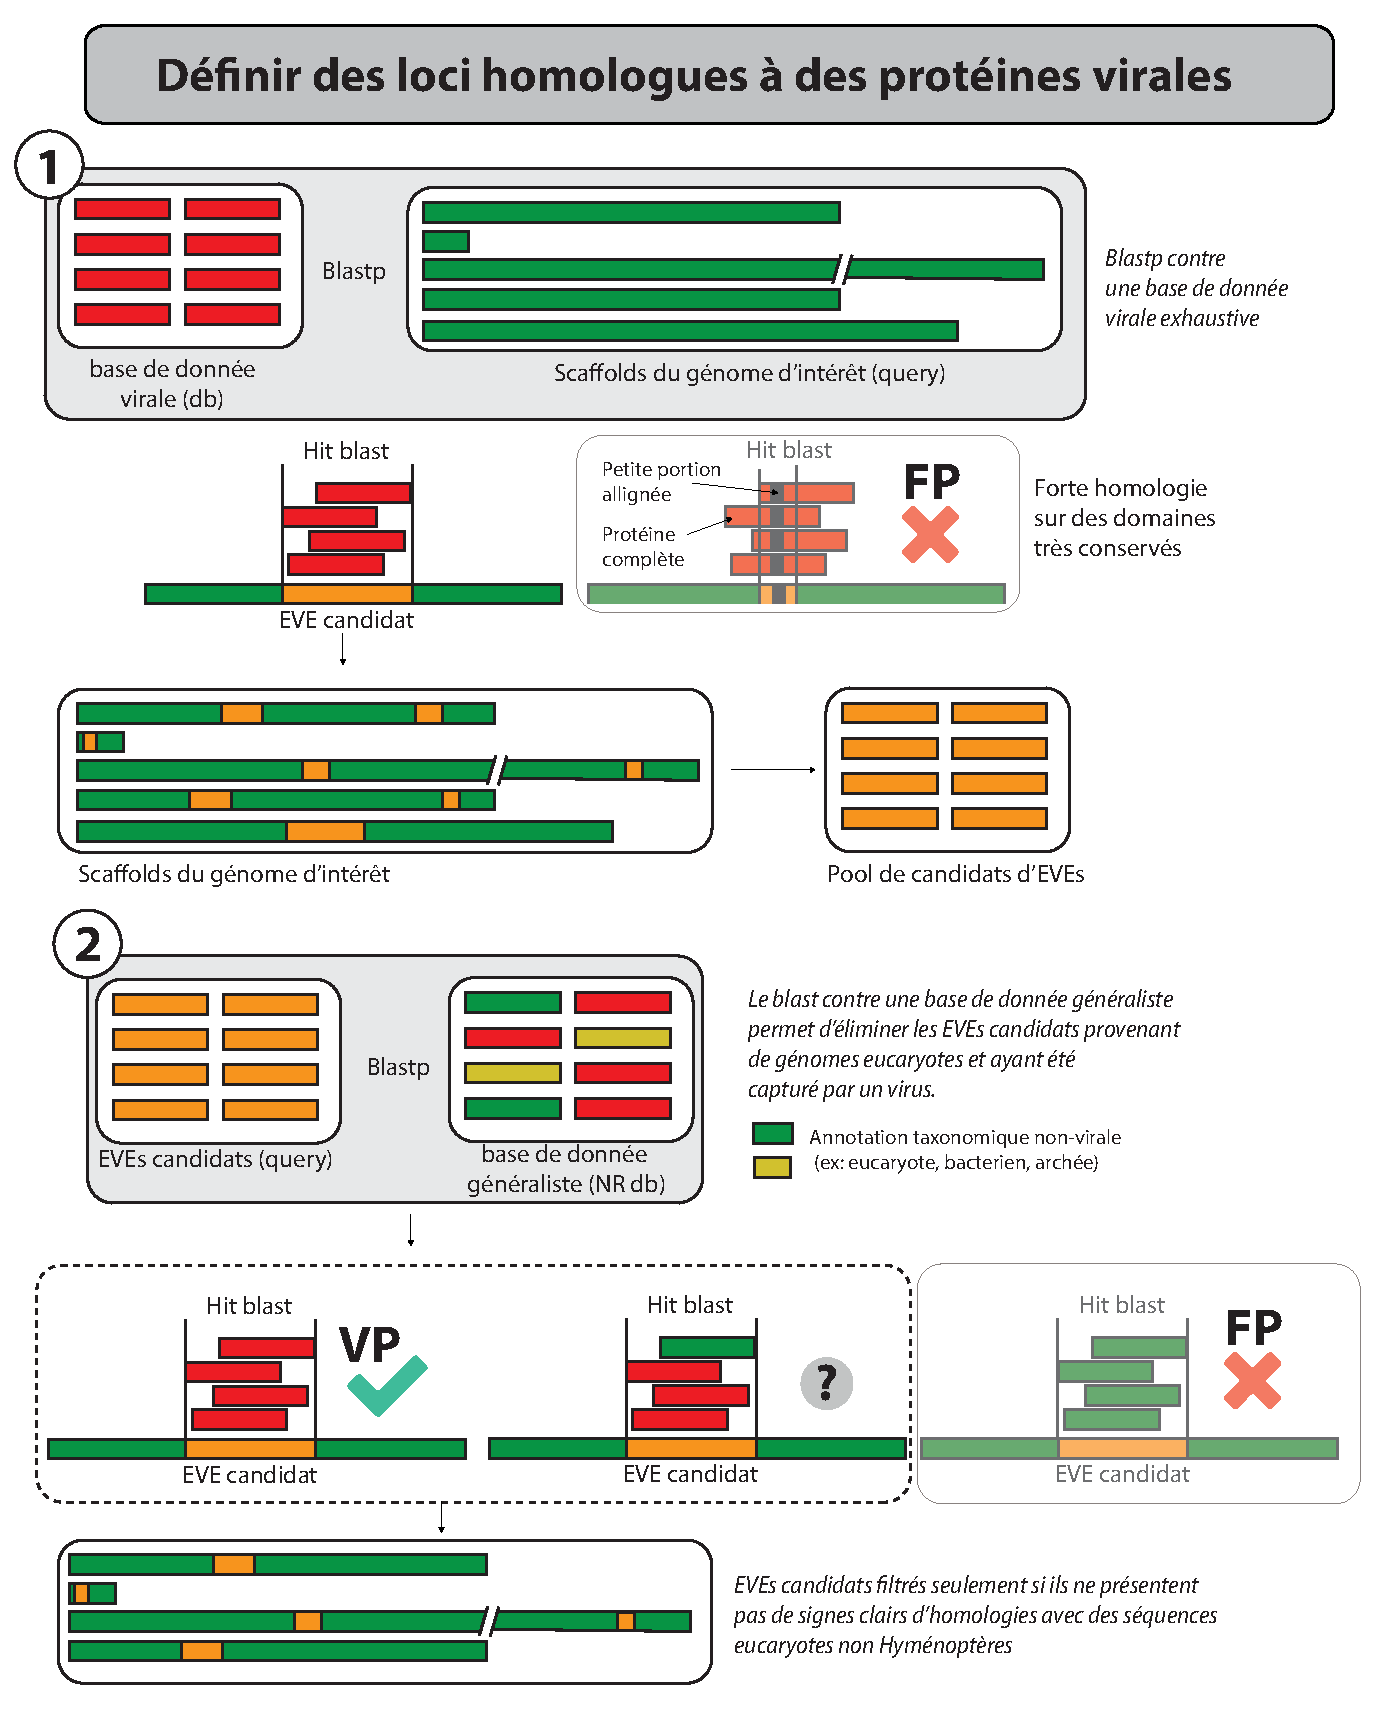
\includegraphics[width=\linewidth,height=\textheight,keepaspectratio]{PhD-master/figures/Methods_Homologie_virale.pdf}
\caption[Methode:Schéma de recherche d'homologie de séquence]{\textbf{Recherche d'homologie de séquence.}}
\label{figure:Methods_Homologie_virale}
\end{figure}

\subsection{Appuyer l'hypothèse d'endogénisation}

Définir la présence d'homologie de séquences entre des loci d'un assemblage et des protéines virales ne suffit pas pour appuyer l'hypothèse d'une intégration virale. Et la raison principale tient au fait qu'une proportion des reads séquencés d'un organisme d'intérêt peut provenir en réalité d'entités biologiques libres que nous pourrions appeler des "contaminants" \citep{steinegger_terminating_2020}. Ces contaminants peuvent provenir de deux sources, soit d'une contamination de laboratoire (c-à-d qu'une entité biologique a été introduite par erreur dans l'échantillon avant séquençage), soit d'une contamination dite "naturelle" qui correspondrait à la présence réelle d'un autre organisme tel qu'un virus ou une bactérie dans les tissus de l'espèce d'intérêt (\figurename{\ref{figure:Contamination}}). 

\begin{figure}[!htpb]
\captionsetup{font=footnotesize}
 \centering
  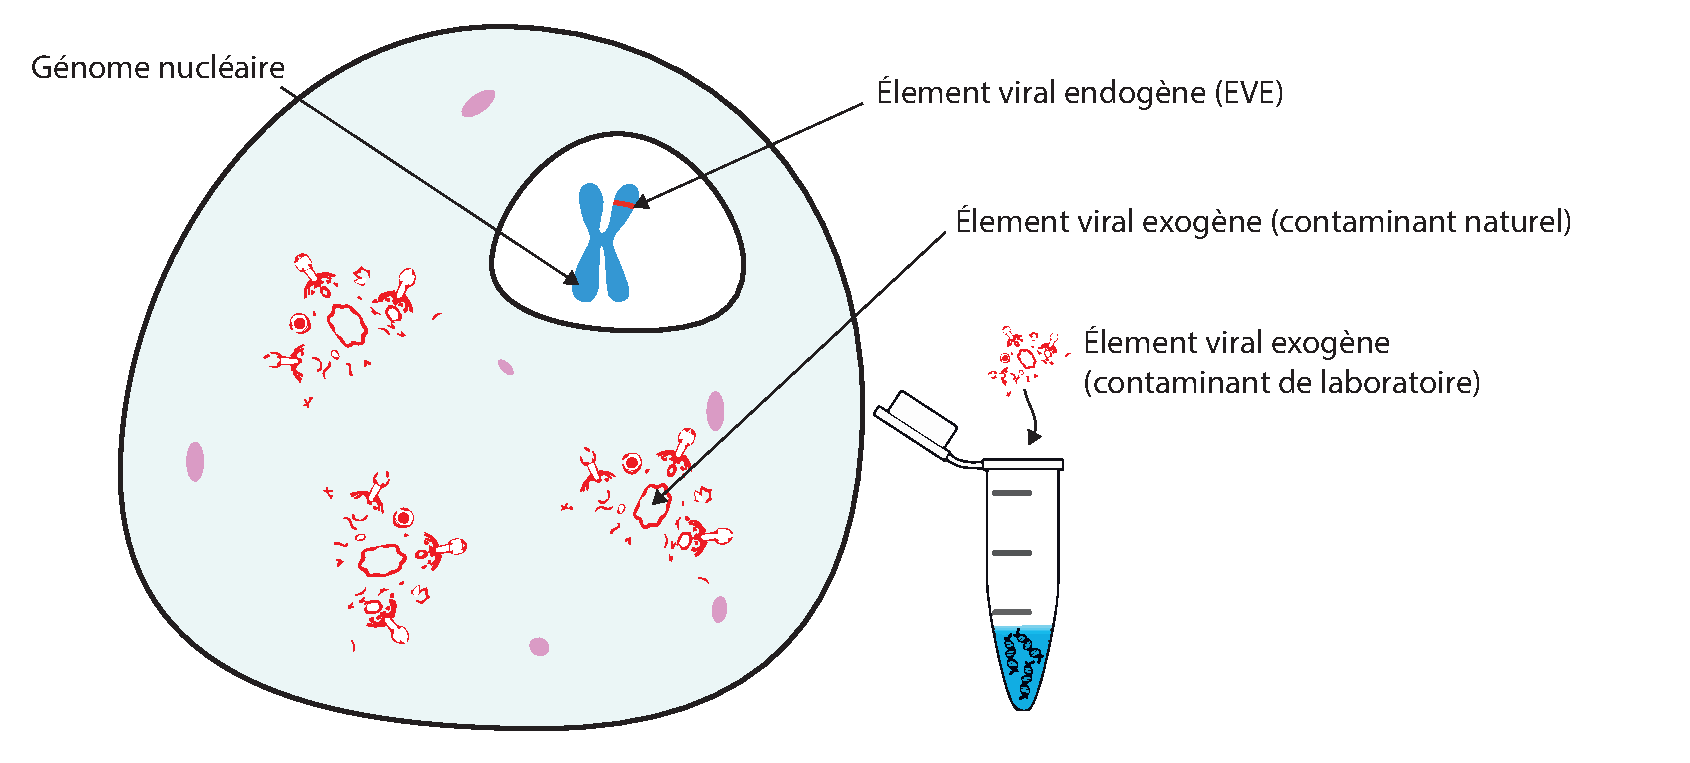
\includegraphics[width=\linewidth,height=\textheight,keepaspectratio]{PhD-master/figures/Contamination.pdf}
\caption[Methode:Schéma de différents types de contaminants et éléments viraux réellement endogénisés]{\textbf{Schéma de différents types de contaminants et éléments viraux réellement endogénisés}}
\label{figure:Contamination}
\end{figure}

Plusieurs éléments nous permettent de placer ces contigs dans l'une ou l'autre des catégories : 

\begin{itemize}

    \item Une façon d'exclure les contigs contaminants consiste à rechercher la présence de gènes eucaryotes et d'éléments transposables dans les contigs contenant des EVEs candidates, en partant du principe que leur présence dans un contig viral est peu probable (\figurename{\ref{figure:Methods_EVEs}}-1). En effet, si de nombreux gènes typiques eucaryotes sont retrouvés le long des contigs, ces observations permettent d'appuyer l'hypothèse que ce contig est bien d'origine eucaryote. Néanmoins, certains virus tels que les grands virus à ADN sont connus pour capturer régulièrement des gènes de leurs hôtes eucaryotes \citep{irwin_systematic_2022}. Aussi, cet argument ne se suffit pas à lui-même. Du côté des éléments transposables, il a été démontré que très peu de génomes viraux contiennent des éléments transposables \citep{miller_virus_1982,gilbert_population_2014,gilbert_continuous_2016,gilbert_viruses_2017,loiseau_wide_2020} car les insertions de TE sont pour la plupart délétères et sont donc rapidement éliminées par la sélection négative \citep{gilbert_continuous_2016, gilbert_viruses_2017}. 

    \item L'argument le plus puissant est sans doute la taille des contigs comme utilisé dans plusieurs études \citep{gilbert_diversity_2022,shen_tempo_2018,li_hgt_2022-1} (\figurename{\ref{figure:Methods_EVEs}}-2). Cette approche se base sur le fait qu'un contig suffisamment grand en taille devrait excéder la taille possible d'un contig viral, et ainsi écarter l'hypothèse d'un contig virale exogène. Cette approche a malgré tout quelques limites. Premièrement, elle est intéressante lorsque l'ont travail sur des génomes très bien assemblés qui permettent d'obtenir des contigs suffisamment grands et ne pas écarter un trop grand nombre de vrais positifs, car les EVEs se trouvent dans des contigs trop petits. De plus, il existe probablement une relation étroite entre la présence d'ETs et la distribution des EVEs le long du génome, or, nous savons que les régions riches en éléments transposables seront beaucoup plus fragmentées le long du génome lors de l'assemblage, spécialement lorsque les techniques de séquences sont basées sur des reads courts \citep{peona_identifying_2021}. Enfin, une autre limitation peut également provenir d'un mauvais assemblage de contig qui assemblerait deux entités génomiques telles qu'un contig de l'insecte et un contig d'un virus ou d'une bactérie par exemple. De tels mauvais assemblages peuvent se produire si très peu de reads mappent en un point et qu'une chute de couverture est observée. Des logiciels tels que MEC permettent de réparer ces mauvais assemblages \citep{wu_mec_2020}.

    \item Il est également possible de se baser sur l'hypothèse d'abondance en reads qui peut être un proxy de l'abondance d'une entité biologique dans les tissus lors de l'assemblage. En effet, les reads qui proviennent des contigs eucaryotes devraient avoir une couverture différente des reads qui découlent des contigs d'entités virales. Dans un exemple, nous voyons clairement que la couverture des contigs viraux (en rouge) est significativement au-dessus de la couverture des reads qui proviennent des contigs eucaryotes (en bleu) (\figurename{\ref{figure:Methods_EVEs}}-3). Ces observations sont également vérifiables pour d'autres entités telles que des bactéries \citep{di_giovanni_behavior-manipulating_2020,burke_presence_2021}. Ainsi, il est possible de mener cette analyse en mappant de préférence les reads d'où provient l'assemblage d'origine, puis de construire une distribution, observée, de couvertures provenant de contigs dont on est certains qu'ils proviennent de l'insecte. De tels contigs peuvent être ceux qui contiennent par exemple un ou plusieurs gènes BUSCOs (les gènes BUSCOs sont des gènes en copie unique universellement présents sous forme d'orthologues au sein d'un groupe en particulier : par exemple les arthropodes \citep{simao_busco_2015}). Cette distribution de couverture BUSCO représente une distribution de la profondeur typique attendue sous l'hypothèse H0 (un contig appartenant au génome de l'insecte). Aussi, pour chaque contig contenant un EVE candidat, il est possible de calculer la valeur p correspond à la proportion de valeurs de profondeur de contigs BUSCOs qui étaient plus extrêmes que celle observée dans le contig candidat (test bilatéral). Dans un tel test, nous rejetons l'hypothèse H0 lorsque cette probabilité est inférieure à 5\%. Cette approche a néanmoins ses limites, car il est possible qu'une entité virale (les virus dsDNA par exemple) puisse approcher la couverture virale moyenne de l'insecte à un point qu'il est difficile de trancher, tel que chez \textit{Dolichomitus} pour lequel des contigs contenant des gènes viraux ont une couverture très légèrement significativement supérieure aux contigs de l'insecte \citep{burke_deep_2012}. Enfin, une autre limitation peut provenir de l'impact d'éléments répétés aux alentours des EVEs, qui par leur nature répétée peuvent au moment du mapping gonfler de manière artificiel la couverture du contig. Un tel biais peut néanmoins être évité en utilisant plutôt la médiane que la moyenne pour rendre compte de la couverture globale d'un contig. 

    \item Enfin, d'autres pistes non développées durant mon travail de thèse, tirées des caractéristiques connues des génomes viraux, peuvent nous permettre d'évaluer leur caractère exogène. Par exemple, la densité en gène des génomes de virus est forte compte tenu des fortes pressions de sélections que leurs génomes subissent \citep{mahmoudabadi_comprehensive_2018}. Néanmoins, ce caractère n'est pas forcément discriminant puisqu'il peut arriver que des régions du génome des insectes soient également fortement denses en gènes. Le contenu en G+C peut également être un facteur intéressant à observer et peut tout comme la couverture discriminer plusieurs entités biologiques. Seulement, le taux de G+C est très hétérogène le long du génome, ce qui peut rendre difficile son interprétation, mais est très utile pour représenter les données comme dans un plot de la couverture et du G+C\% des contigs (\figurename{\ref{figure:Methods_EVEs}}-3). La composition des EVEs eux-mêmes peut être analysée, avec la présence d'introns dans les séquences. En effet, les gènes de virus à ARN ne présentent en général pas d'introns, bien qu'il soit bien connu que certains génomes viraux eucaryotes, semblables aux génomes de leurs hôtes, contiennent des gènes avec des introns \citep{mahmoudabadi_comprehensive_2018}. Nous pourrions également étudier l'usage des codons des gènes dans un scaffold qui devrait être spécifique selon les entités (c'est-à-dire une fréquence inégale des codons alternatifs qui spécifient le même acide aminé). Seulement, il a également été mis en évidence que les protéomes des virus sont adaptés aux protéomes de leurs hôtes en présentant une utilisation similaire des codons \citep{tian_adaptation_2018,bahir_viral_2009}. De plus, lorsqu'un gène viral est endogénisé et qu'il devient fonctionnel, on peut s'attendre à ce que ce gène s'adapte au cours des générations, à l'usage du codon du génome hôte. 
    Pour terminer, un argument intéressant pour soutenir la thèse d'une intégration peut être celle de retrouver un hit convaincant avec une protéine de virus au génome ARN (simple brin ou double brins), alors même que les reads proviennent de séquençage ADN. En effet, les virus à ARN ne connaissent pas de phase ARN dans leur réplication (sauf rétrovirus), retrouver ainsi un hit dans des données ADN veut donc dire que ce virus est bien intégré dans la matrice ADN de l'hôte. Seulement, quelques contre-exemples émergent dans la littérature à ce propos. Une explication possible pourrait provenir de la transcription inverse des génomes ARN en ADNc par un rétrotransposon ou un rétrovirus hôte endogène \citep{klenerman_non-retroviral_1997} suite à une infection. Ce type de mécanisme, encore mal connu, a été reconnu comme étant impliqué dans la réponse immunitaire antivirale chez le moustique et la drosophile \citep{goic_rna-mediated_2013,goic_virus-derived_2016,tassetto_control_2019}, qui, en outre, peut être transmise à la descendance \citep{mondotte_evidence_2020}. De plus, une analyse a montré que la plupart des formes d'ADN des virus à ARN possèdent des rétrotransposons à répétition terminale longue (LTR) dans leur région \citep{goic_virus-derived_2016}.\\
\end{itemize}

Au final, comme nous venons de le constater, une seule métrique pour appuyer l'hypothèse d'endogénisation n'est généralement pas suffisante, car elles s'accompagnent toutes de limitations. Aussi, il est sans doute préférable de plutôt croiser ces métriques pour approcher des degrés de confiance envers le caractère endogénisés des EVEs. De tels "échelles de confiances" peuvent par exemple correspondre à une échelle de A à D pour des contigs probablement d'origine eucaryotes, à F et X pour des contigs qui devraient plutôt appartenir à des entités exogènes (\figurename{\ref{figure:Methods_EVEs}}-4). 
    

\begin{figure}[!htpb]
\captionsetup{font=footnotesize}
 \centering
  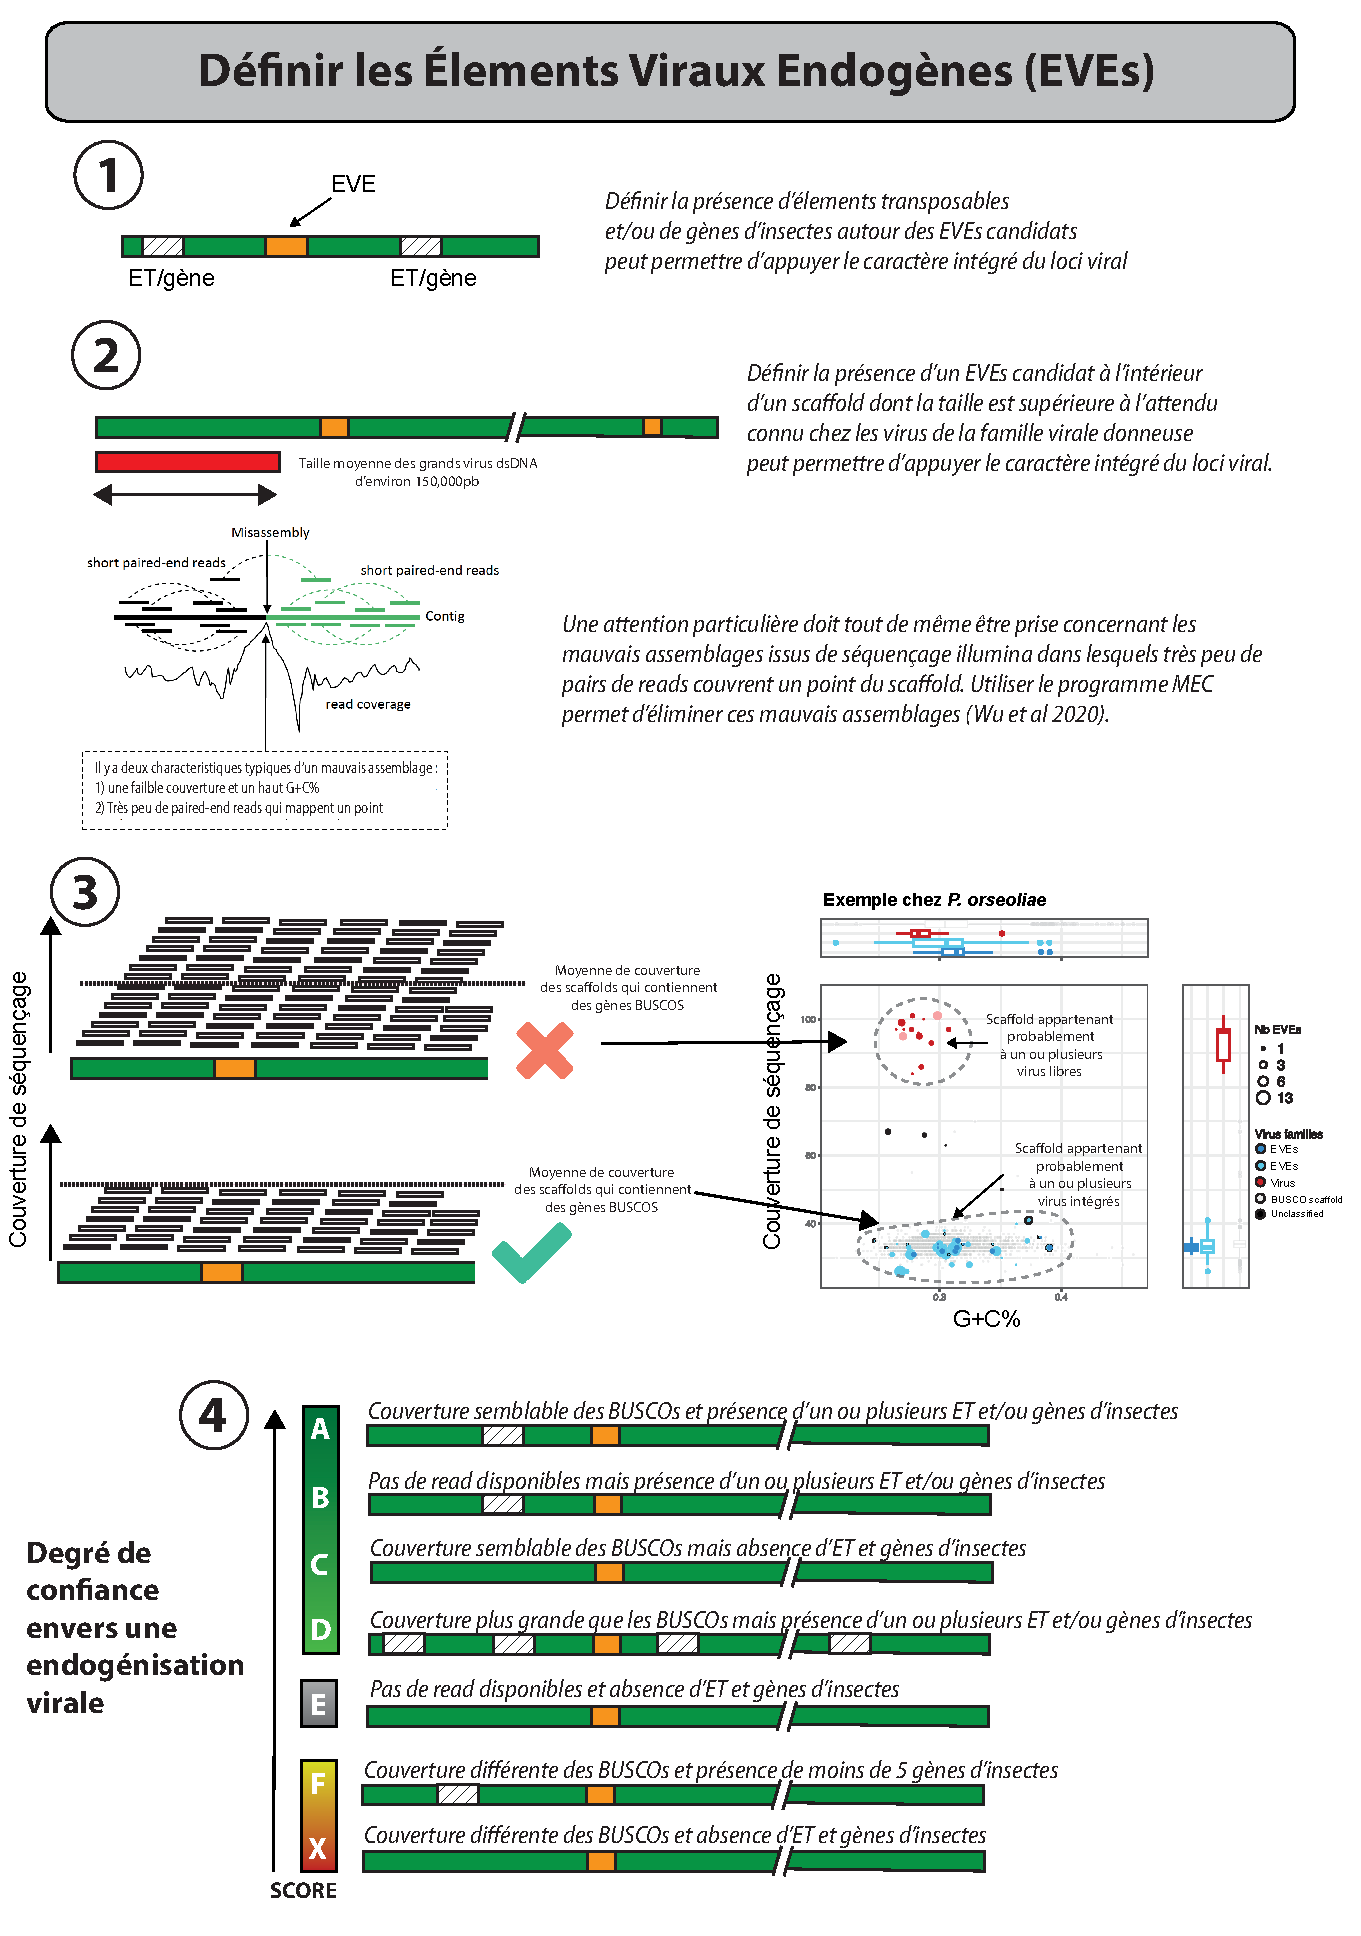
\includegraphics[width=\linewidth,height=\textheight,keepaspectratio]{PhD-master/figures/Methods_EVEs.pdf}
\caption[Methode:Définition des éléments viraux endogénisés]{\textbf{Définition des éléments viraux endogénisés}.}
\label{figure:Methods_EVEs}
\end{figure}


\section{Étudier l'histoire évolutive des EVEs}

Nous l'avons vu dans quelques exemples en introduction, la présence de plusieurs EVEs peut être la conséquence d'histoire évolutive complexes dans lesquelles les gènes viraux endogènes ont été transmis verticalement sur plusieurs générations depuis un ancêtre commun. Afin d'étudier ces histoires évolutives, une première approche peut-être de rassembler les EVEs candidats partageant des homologies de séquences en clusters (\figurename{\ref{figure:Histoire_EVEs-domestication}}-1). Aligner ensuite les séquences de ces clusters (\figurename{\ref{figure:Histoire_EVEs-domestication}}-2) permet d'obtenir une matrice protéique utile pour inférer un arbre phylogénétique(\figurename{\ref{figure:Histoire_EVEs-domestication}}-3). Cet arbre phylogénétique est indispensable pour rendre compte de l'histoire évolutive des gènes d'intérêt, car il capture les liens phylogénétiques entre les séquences virales endogénisés d'une ou plusieurs espèces (orange) et les séquences des virus libres dans les bases de données (rouge). Cet à travers cet arbre que nous pouvons essayer d'inférer les évènements d'endogénisations (\figurename{\ref{figure:Histoire_EVEs-domestication}}-4). 

\begin{figure}[!htpb]
\captionsetup{font=footnotesize}
 \centering
  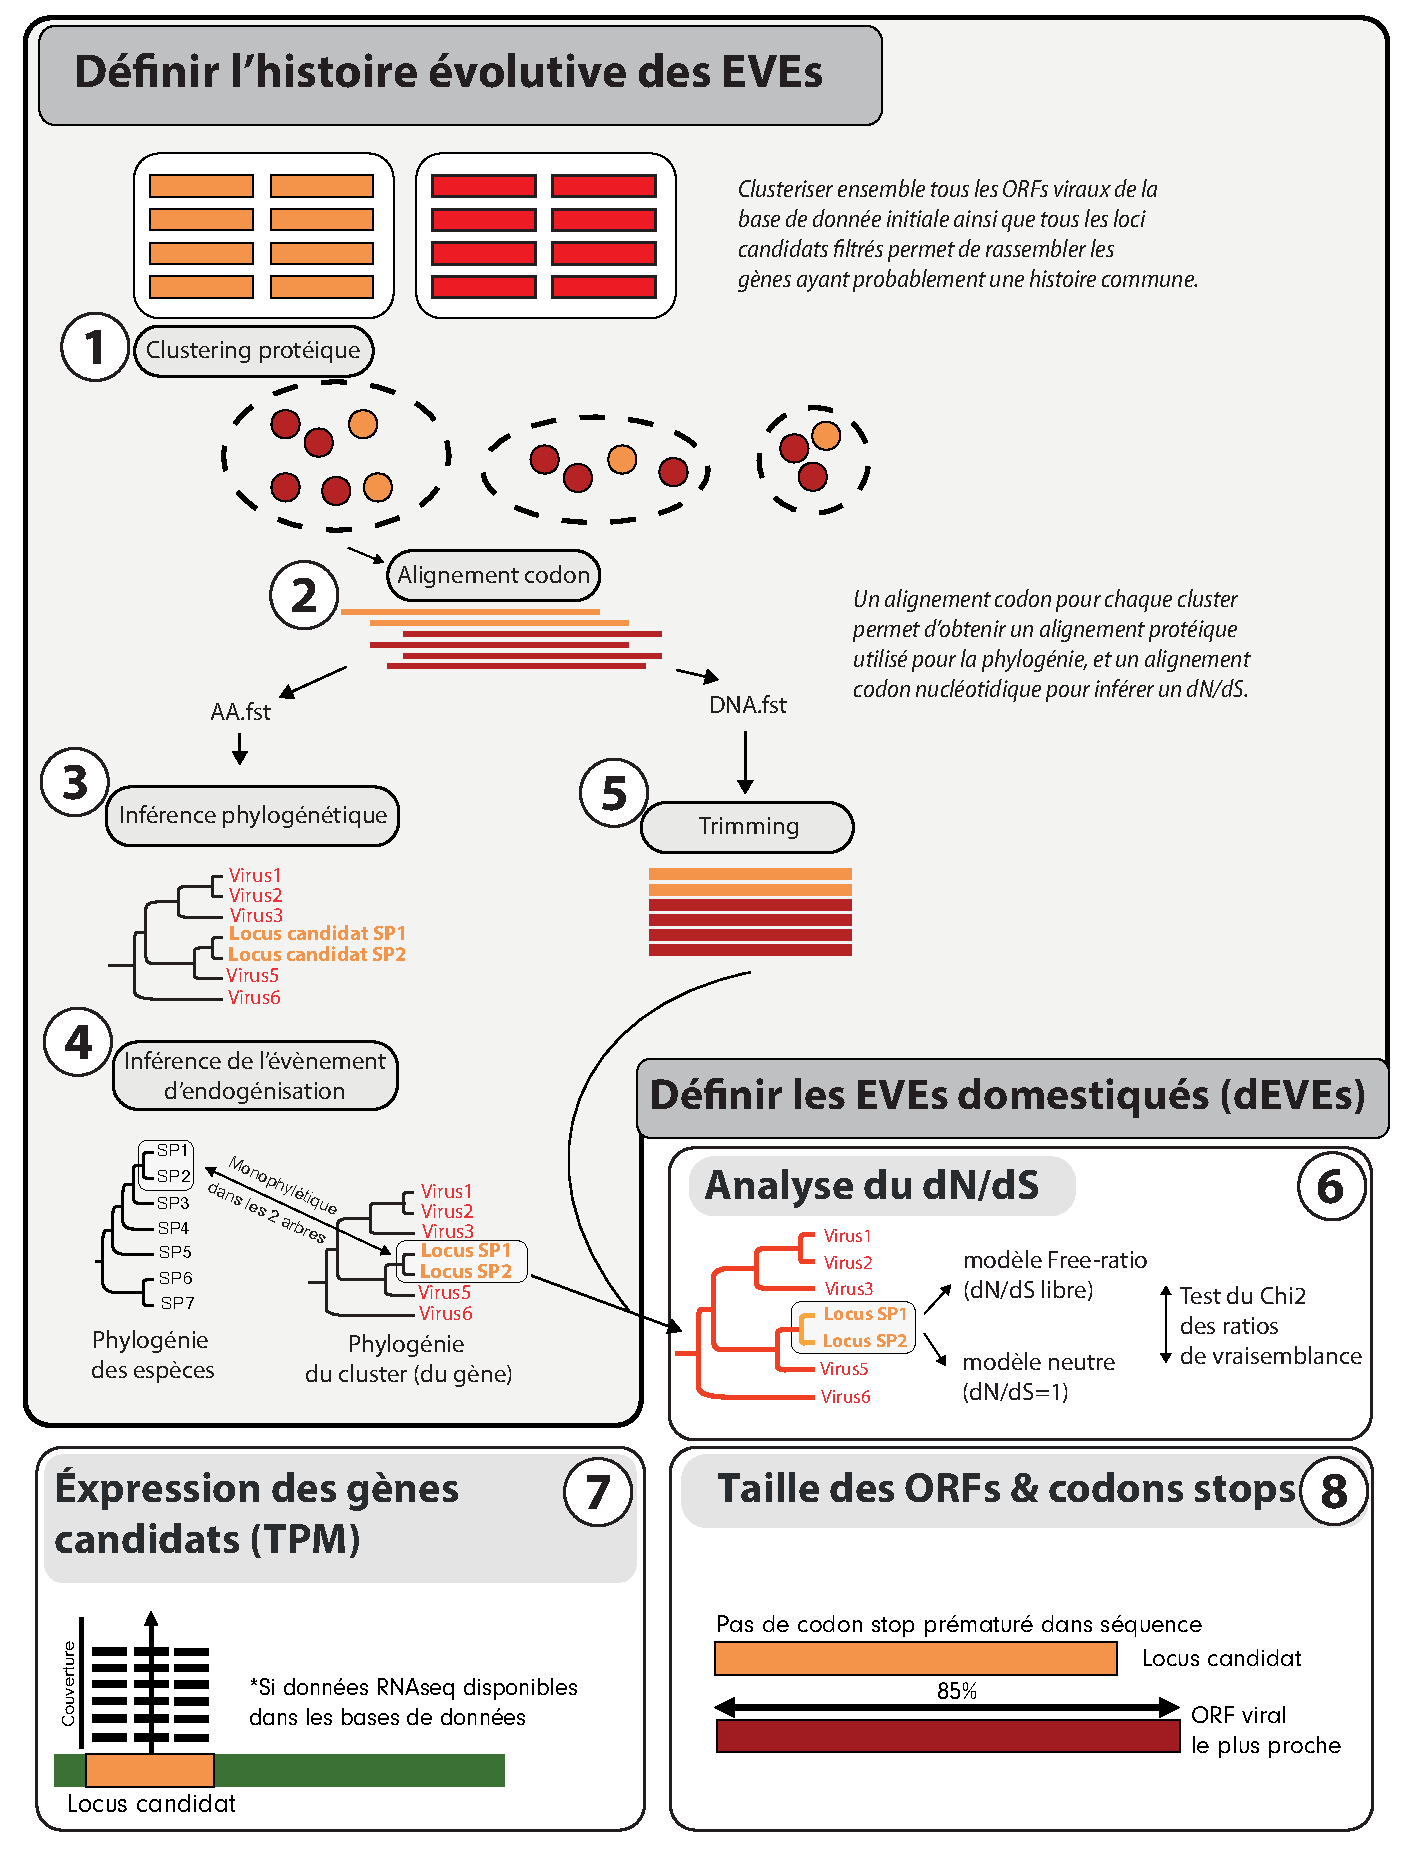
\includegraphics[width=\linewidth,height=\textheight,keepaspectratio]{PhD-master/figures/Histoire_EVEs-domestication.pdf}
\caption[Methode:Illustration de l'histoire évolutive de l'acquisition des EVEs et dEVEs]{\textbf{Illustration de l'histoire évolutive de l'acquisition des EVEs et d'inférence de leur domestication}.}
\label{figure:Histoire_EVEs-domestication}
\end{figure}

\section{Inférer les évènements d'endogénisations}

Inférer un évènement à partir d'un EVE peut être simple lorsque cet EVE provient effectivement d'un seul évènement d'endogénisation passé (\figurename{\ref{figure:Types_evenements}}-1). Lorsqu'il existe plusieurs EVEs inférés dans un génome, en revanche, ce nombre ne permet pas d'en déduire directement le nombre d'évènements d'endogénisaton indépendants. En effet, la présence de plusieurs EVEs peut provenir d'un seul évènement d'endogénisation correspondant aux gènes du génome viral, ou bien même correspondre à un ou plusieurs gènes viraux ayant subi des épisodes de duplication post-endogénisation (\figurename{\ref{figure:Types_evenements}}-2), d'un seul évènement chez l'ancêtre commun de plusieurs espèces, et dont les EVEs ont été ensuite transmit de manière verticale aux descendants (\figurename{\ref{figure:Types_evenements}}-3), ou bien provenir de plusieurs évènements d'endogénisations indépendantes (\figurename{\ref{figure:Types_evenements}}-4).

Face à ces différents cas de figures, plusieurs méthodes peuvent nous permettre d'inférer des évènements le long des phylogénies d'espèces.

\begin{itemize}

    \item Pour détecter les évènements de type 2 (\figurename{\ref{figure:Types_evenements}}-2), il est possible de se baser sur la présence de plusieurs EVEs le long d'un même scaffold. Ainsi, la promiscuité entre des EVEs peut nous permettre d'imaginer qu'ils proviennent d'un même évènement d'endogénisation. Seulement, plus le génome étudié sera fragmenté, plus il sera difficile d'utiliser cette approche. 
    
    \item Pour discriminer plusieurs évènements indépendants comme le type 3 (\figurename{\ref{figure:Types_evenements}}-3), une manière de faire peut-être de rassembler au sein du même évènement les EVEs provenant de virus de la même famille (bleu et rose). L'assignation des familles virales peut par exemple se baser sur l'assignation taxonomique la plus proche lors d'un blast, ou bien à l'aide de l'assignation taxonomique du dernier ancêtre commun des hits les plus proches tel que développé dans l'approche 2bLCA \cite{ingamp_exploring_2013}. Aussi, il est peu probable qu'un même évènement unique présente des assignations taxonomiques au niveau de la famille qui sont différents. Seulement, l'assignation taxonomique a ses limites lorsque les hits dans les bases de données sont des séquences inconnues (et ils sont nombreux \citep{mirdita_fast_2021}), ou bien lorsque plusieurs évènements ont eu lieu au sein de la même famille virale, dans ce cas, l'algorithme sous-estimera le nombre d'évènements. Malheureusement, utiliser un autre degré de hiérarchie tel que les sous-familles virales peut devenir aussi problématique puisqu'il peut cette fois-ci surestimer le nombre d'événements lorsque les assignations taxonomiques ne sont pas aussi précises. 
    
    \item Pour discriminer un seul évènement commun à plusieurs espèces comme le type 4 (\figurename{\ref{figure:Types_evenements}}-4), une manière de faire peut-être de placer les évènements le long de la phylogénie des espèces et de vérifier si les espèces qui présentent des insertions pour une même famille virale sont effectivement proches phylogénétiquement (ici SP1 et SP2 sont par exemple des espèces sœurs, il est donc fort probable qu'elles aient hérité ces EVEs de leur ancêtre commun). Cet algorithme peut autoriser des pertes chez quelques espèces pour prendre en compte la possibilité de perte chez quelques espèces descendantes d'un ancêtre commun d'un clade. Une limite à cette approche peut provenir des cas où un évènement a bien eu lieu chez l'ancêtre commun de deux espèces, mais que des pertes sont observées chez l'une des deux. Dans un tel cas, l'algorithme va inférer deux évènements à part, car il est possible d'imaginer qu'un deuxième épisode d'endogénisation ait eu lieu après le premier, pouvant expliquer à tort ou à raison l'absence d'un gène chez les autres espèces. Par exemple, dans le \hyperref[sec:chap3]{chapitre 3}, l'algorithme aurait eu raison d'inférer deux évènements chez les Eucoilini qui ne correspondent pas a priori à des pertes, mais bien deux évènements indépendants. 
  
 \end{itemize}  
  
Bien qu'un tel algorithme ne soit pas parfait compte tenu des biais que je viens d'évoquer, il semble fonctionner et inférer correctement des évènements connus le long d'une phylogénie. Par exemple, si on l'utilise pour inférer des évènements chez 4 cas connus d'endogénisations virales observées dans le \hyperref[sec:chap2]{chapitre 2}  (\figurename{\ref{figure:Virus_arthropods_phylogeny}}) : (1 évènement unique chez \textit{V.canescens} \citep{pichon_recurrent_2015}, un évènement unique chez \textit{F.arisanus} \citep{burke_rapid_2018}, 1 évènement partagé par deux espèces de microgastroïdes chez \textit{M.demolitor} et \textit{C.vestalis} \citep{bezier_polydnaviruses_2009} et 1 évènement partagé par trois espèces chez \textit{L.boulardi}, \textit{L.clavipes} et \textit{L.heterotoma} (Di Giovanni et al., 2020), on s'aperçoit que tous les évènements sont correctement inférés, mais qu'en revanche, 2 évènements sont inférés en plus dans le cas des microgastroïdes. Ceci étant dû au biais que je développe juste avant dans lequel un EVE est absent à deux reprises chez l'une des deux espèces.

\begin{figure}[!htpb]
\captionsetup{font=footnotesize}
 \centering
  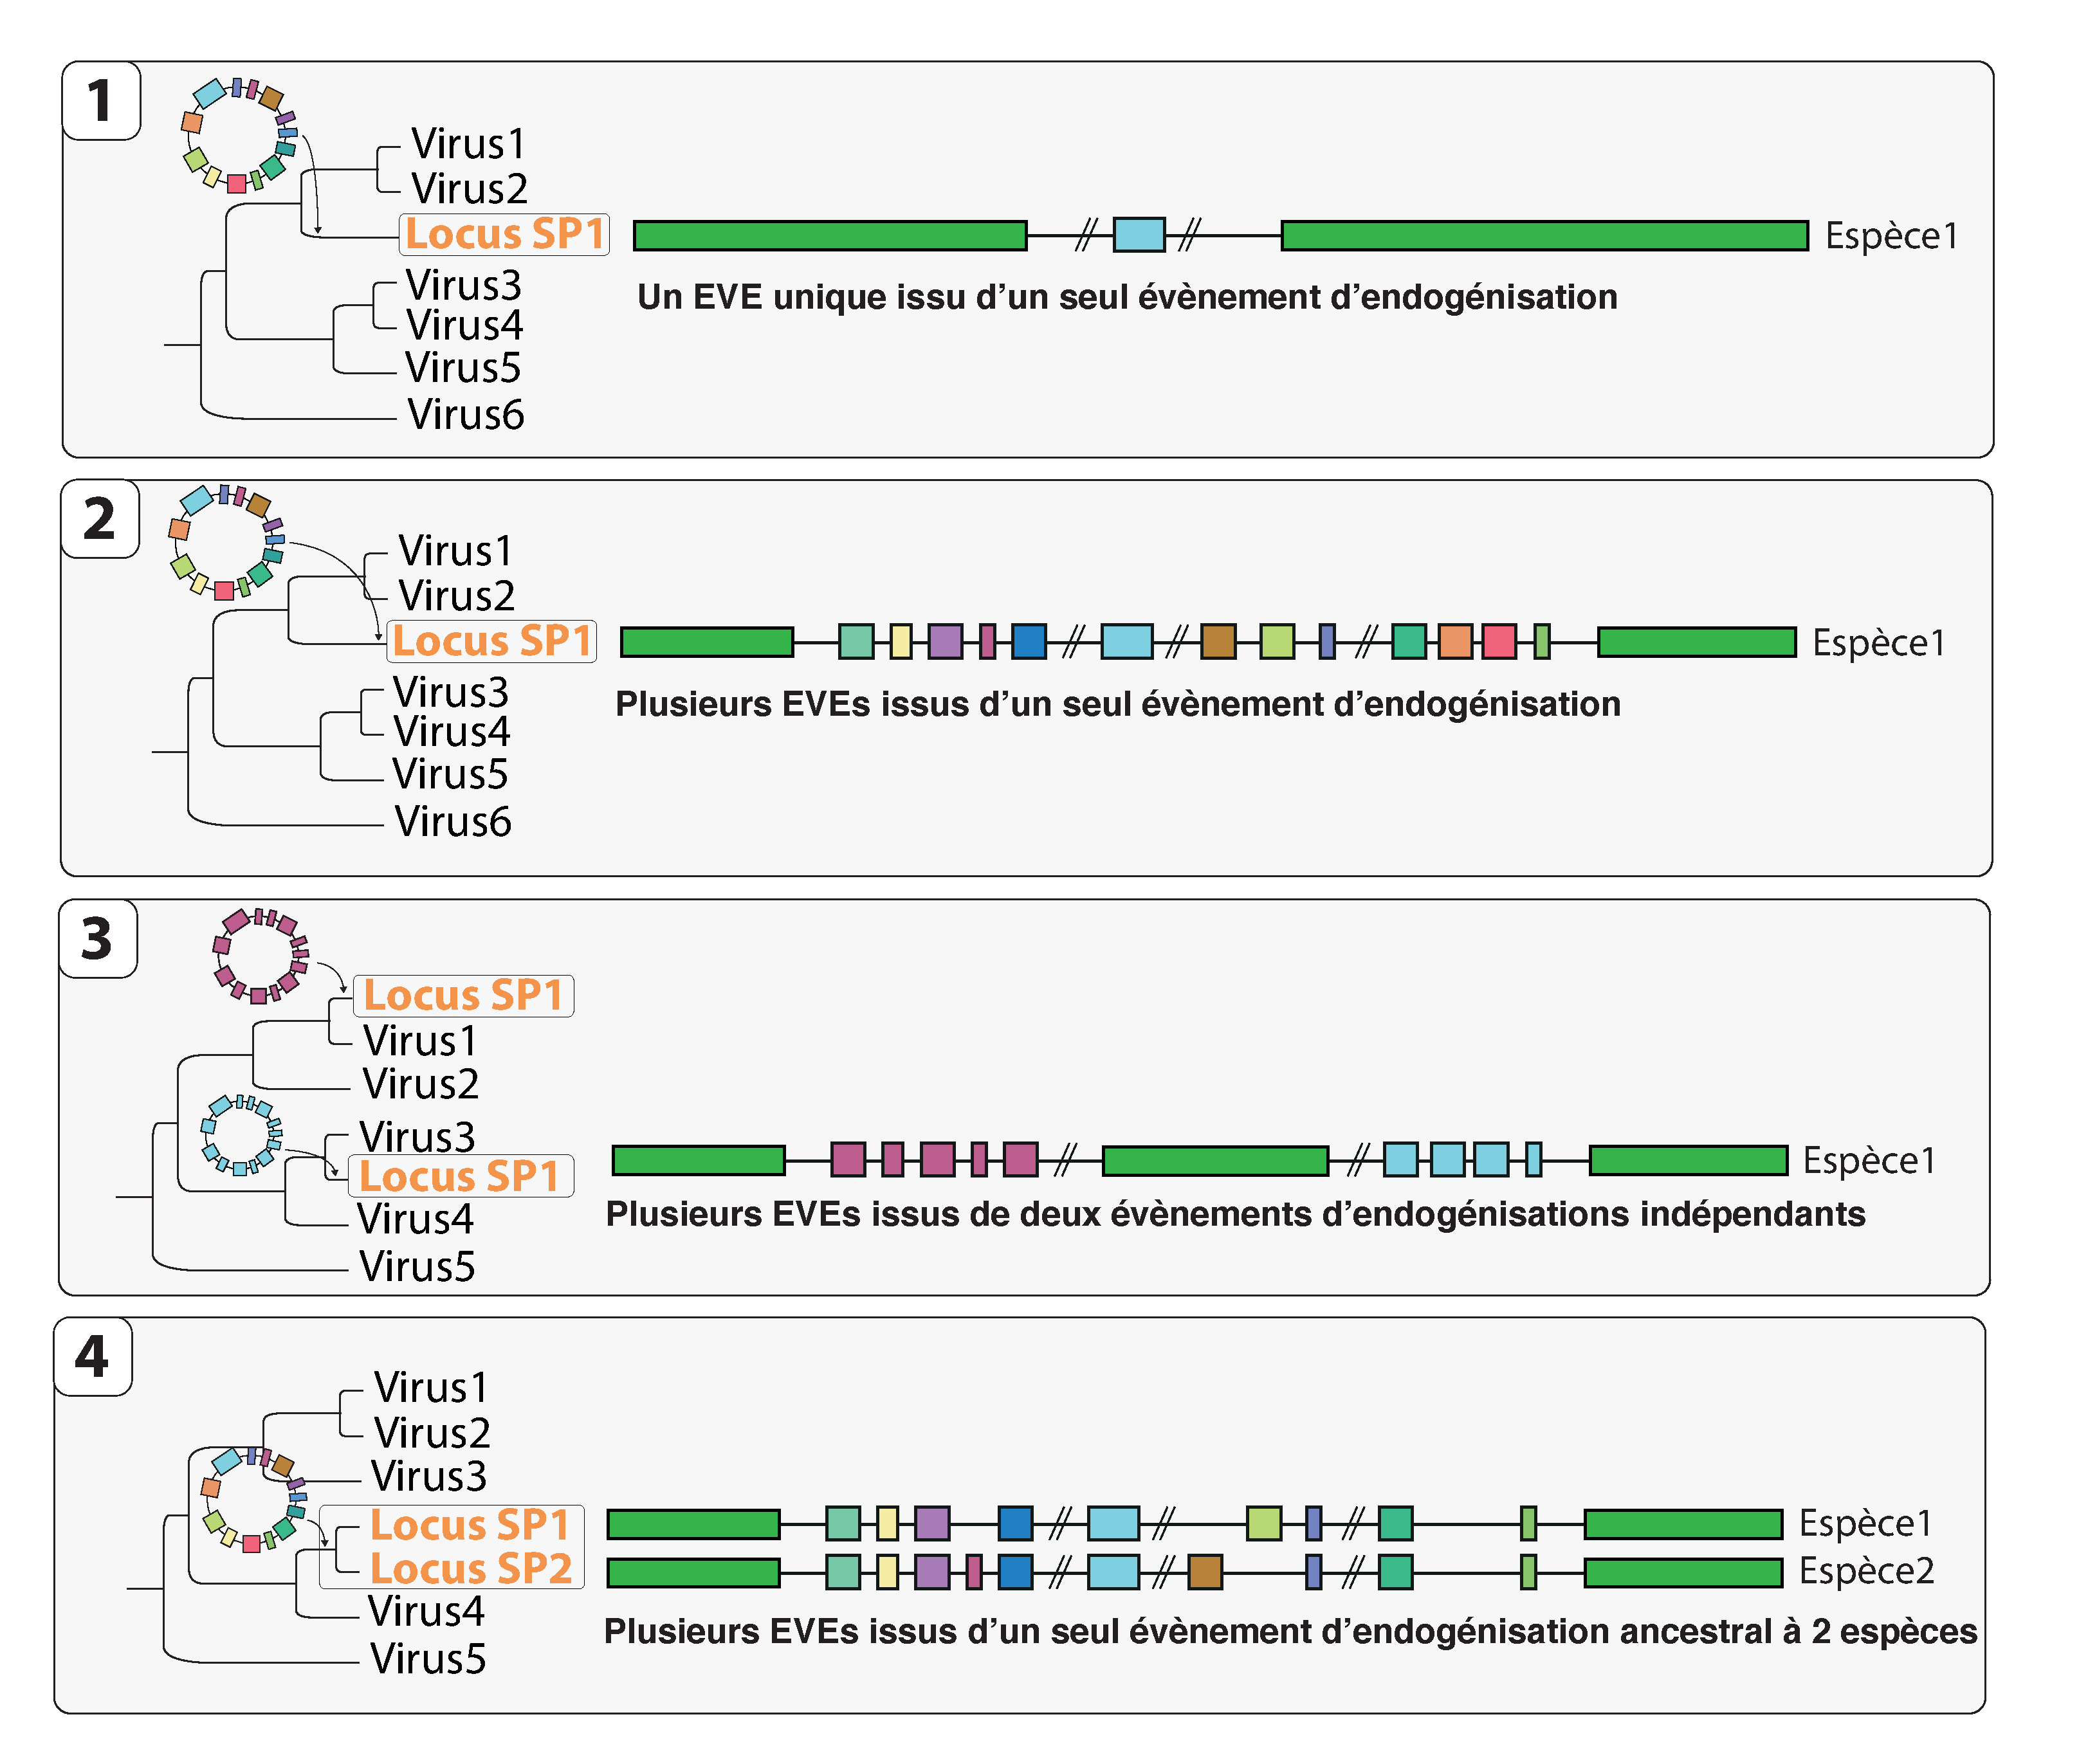
\includegraphics[width=\linewidth,height=\textheight,keepaspectratio]{PhD-master/figures/Types_evenements.pdf}
\caption[Methode:Définition des divers types d'évènements d'endogénisation]{\textbf{Définition des divers types d'évènements d'endogénisation}.}
\label{figure:Types_evenements}
\end{figure}

Enfin, une dernière limitation peut provenir de l'inférence phylogénétique des gènes en elle-même qui peut brouiller l'histoire phylogénétique passée des insertions. En effet, lorsqu'une phylogénie est très mal résolue, alors toutes tentatives d'inférence d'évènements est compromise. Dans mon analyse, nous nous basons sur des métriques comme les scores de bootstraps qui soutiennent des nœuds pour inférer des évènements comme celui de l’exemple de la  (\figurename{\ref{figure:Collapse_de_branche_evenements}}-B). Seulement, si un nœud n'est pas bien soutenu, nous inférons des évènements indépendants, alors qu'il serait envisageable de plutôt collapser les banches faiblement soutenues, et ensuite inférer des évènements, ce qui serait plus parcimonieux en inférant un seul évènement, plutôt que deux indépendants entre deux espèces qui sont pourtant proches phylogénétiquement (\figurename{\ref{figure:Collapse_de_branche_evenements}}-B). 


\begin{figure}[!htpb]
\captionsetup{font=footnotesize}
 \centering
  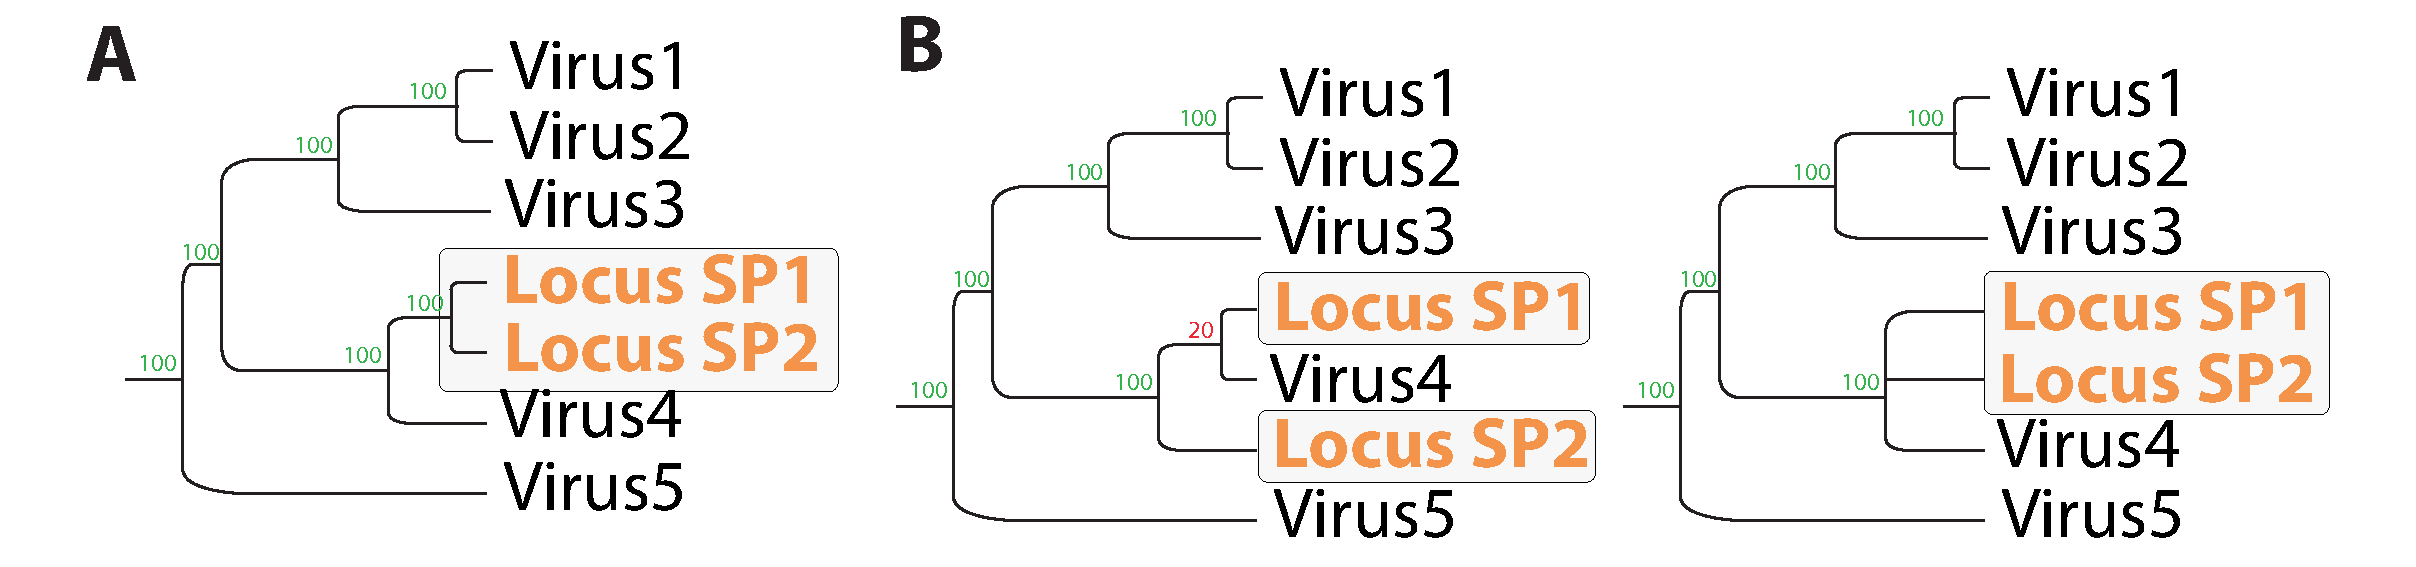
\includegraphics[width=\linewidth,height=\textheight,keepaspectratio]{PhD-master/figures/Collapse_de_branche_evenements.pdf}
\caption[Methode:Exemple d'arbre d'EVE mal résolu]{\textbf{Exemple d'arbre d'EVE mal résolu}.}
\label{figure:Collapse_de_branche_evenements}
\end{figure}


\section{Inférer une domestication des EVEs (dEVEs)}

Une façon de formuler une hypothèse sur la domestication des EVEs (dEVEs) est d'examiner la pression sélective qui s'exerce sur les séquences en estimant le rapport (oméga ou ω) entre le nombre de substitutions non-synonymes par site non-synonyme (\textit{dN)}, dans une période de temps donnée, et le nombre de substitutions synonymes par site synonyme (\textit{dS}) (\figurename{\ref{figure:Histoire_EVEs-domestication}}-6). Ainsi, si les EVEs subissent post-endogénisation une pression de sélection purifiante (\textit{dN/dS} inférieur à 1) ou diversifiante (\textit{dN/dS} supérieur à 1), nous nous attendons à ce que ce rapport s'écarte significativement de 1 (qui est l'évolution neutre du gène avec autant de substitutions synonymes que non-synonymes observés). Ainsi, pour effectuer cette analyse, nous avons besoin de : (i) un alignement codon auquel nous avons au préalable nettoyé (ou trimmé) l'alignement (\figurename{\ref{figure:Histoire_EVEs-domestication}}-5), car il a été observé un effet sur les longueurs de branches des topologies lorsque les séquences ne sont pas "nettoyées", ce qui peut biaiser les analyses et déduire de la sélection à tort. \citep{ranwez_chapter_2020,tan_current_2015}. Et enfin, nous avons besoin de la topologie du gène inférée dans l'étape précédente (\figurename{\ref{figure:Histoire_EVEs-domestication}}-4) accompagné d'une assignation d'évènement le long de la topologie. Cet évènement peut concerner plusieurs branches s'il concerne plusieurs espèces ayant acquis les EVEs depuis leur ancêtre commun (\figurename{\ref{figure:Histoire_EVEs-domestication}}-6). Ainsi, les branches qui seront testées seront les branches dites \textit{forground}. Elles traduiront les pressions de sélections opérées sur le gène viral depuis qu'il est endogénisé dans le génome des hôtes. En marquant ces branches, un modèle de branche calculera différentes valeurs omega (ω) dans les branches \textit{forground} et dans le reste de l'arbre (généralement appelé \textit{backround}) (\figurename{\ref{figure:Collapse_de_branche_evenements}}-B). Puisque cette analyse nécessite au moins deux séquences homologues pour fonctionner, seuls les cas impliquant au moins deux espèces sœurs et/ou une espèce présentant au moins deux paralogues peuvent être utilisés.
Afin d'assurer la qualité des \textit{dN/dS} estimés, nous pouvons (i) tester l'écart significatif par rapport au modèle nul dans lequel les branches du groupe monophylétique ont évolué selon un scénario neutre (test du chi2 carré), (ii) estimer les erreurs standard des estimations du \textit{dN/dS} qui maximisent la vraisemblance (option getSE = 1 dans codeml), et (iii) supprimer les \textit{dN/dS} estimés supérieurs à 10, car l'estimation ne serait pas précise en raison d'une saturation de substitution.

Une limite à l'approche du \textit{dN/dS} peut tout de même se présenter lorsque les évènements que nous inférons sont faux à cause de la présence d'espèces de virus fantômes dans les données (c'est-à-dire des virus non échantillonnés ou bien éteints). Ce genre de limitation peut être typique des familles virales très peu décrites, comme dans le cas des Filamentoviridae que nous voyons dans le \hyperref[sec:chap2]{chapitre 2}, dans lequel une seule espèce de virus représente un groupe viral entier. En effet, dans un cas classique tel que la phylogénie observable du gène (\figurename{\ref{figure:Biais_dNdS}}-A), il peut arriver que l'algorithme infère un évènement ancestral entre deux espèces sœurs, mais qu'en réalité, les deux espèces aient acquis ce gène indépendamment à travers deux virus proches. Par exemple, dans la (\figurename{\ref{figure:Biais_dNdS}}-B), SP1 aurait acquis ce gène d'un proche parent du virus "inconnu 1", tandis que SP2 aurait acquis ce gène d'un proche parent du virus "inconnu 3". Dans un tel scénario, si nous inférons le \textit{dN/dS} sur la phylogénie observée de la (\figurename{\ref{figure:Biais_dNdS}}-A), le \textit{dN/dS} sera biaisé vers un \textit{dN/dS} inférieur à 1 puisque nous capturons dans l'analyse également les forces de sélections opérant sur des branches de virus (en rouge) (\figurename{\ref{figure:Biais_dNdS}}-B). Une manière de s'assurer que la phylogénie observée du gène est bien celle qui est réelle tout comme dans la (\figurename{\ref{figure:Biais_dNdS}}-C) serait ainsi de comparer la distribution des divergences synonymes (\textit{dS}) attendues entre les espèces concernées (bleu) sur plusieurs gènes le long de la phylogénie des espèces (\figurename{\ref{figure:Biais_dNdS}}-A), puis de s'assurer que le \textit{dS} du gène entre les deux espèces du clade tombe dans cette distribution, auquel cas l'hypothèse d'endogénisation depuis l'ancêtre commun est validée (\figurename{\ref{figure:Biais_dNdS}}-C), ou invalidée (\figurename{\ref{figure:Biais_dNdS}}-B). Ceci est malgré tout une piste à exploiter et ne l'a pas été durant ma thèse. 

\begin{figure}[!htpb]
\captionsetup{font=footnotesize}
 \centering
  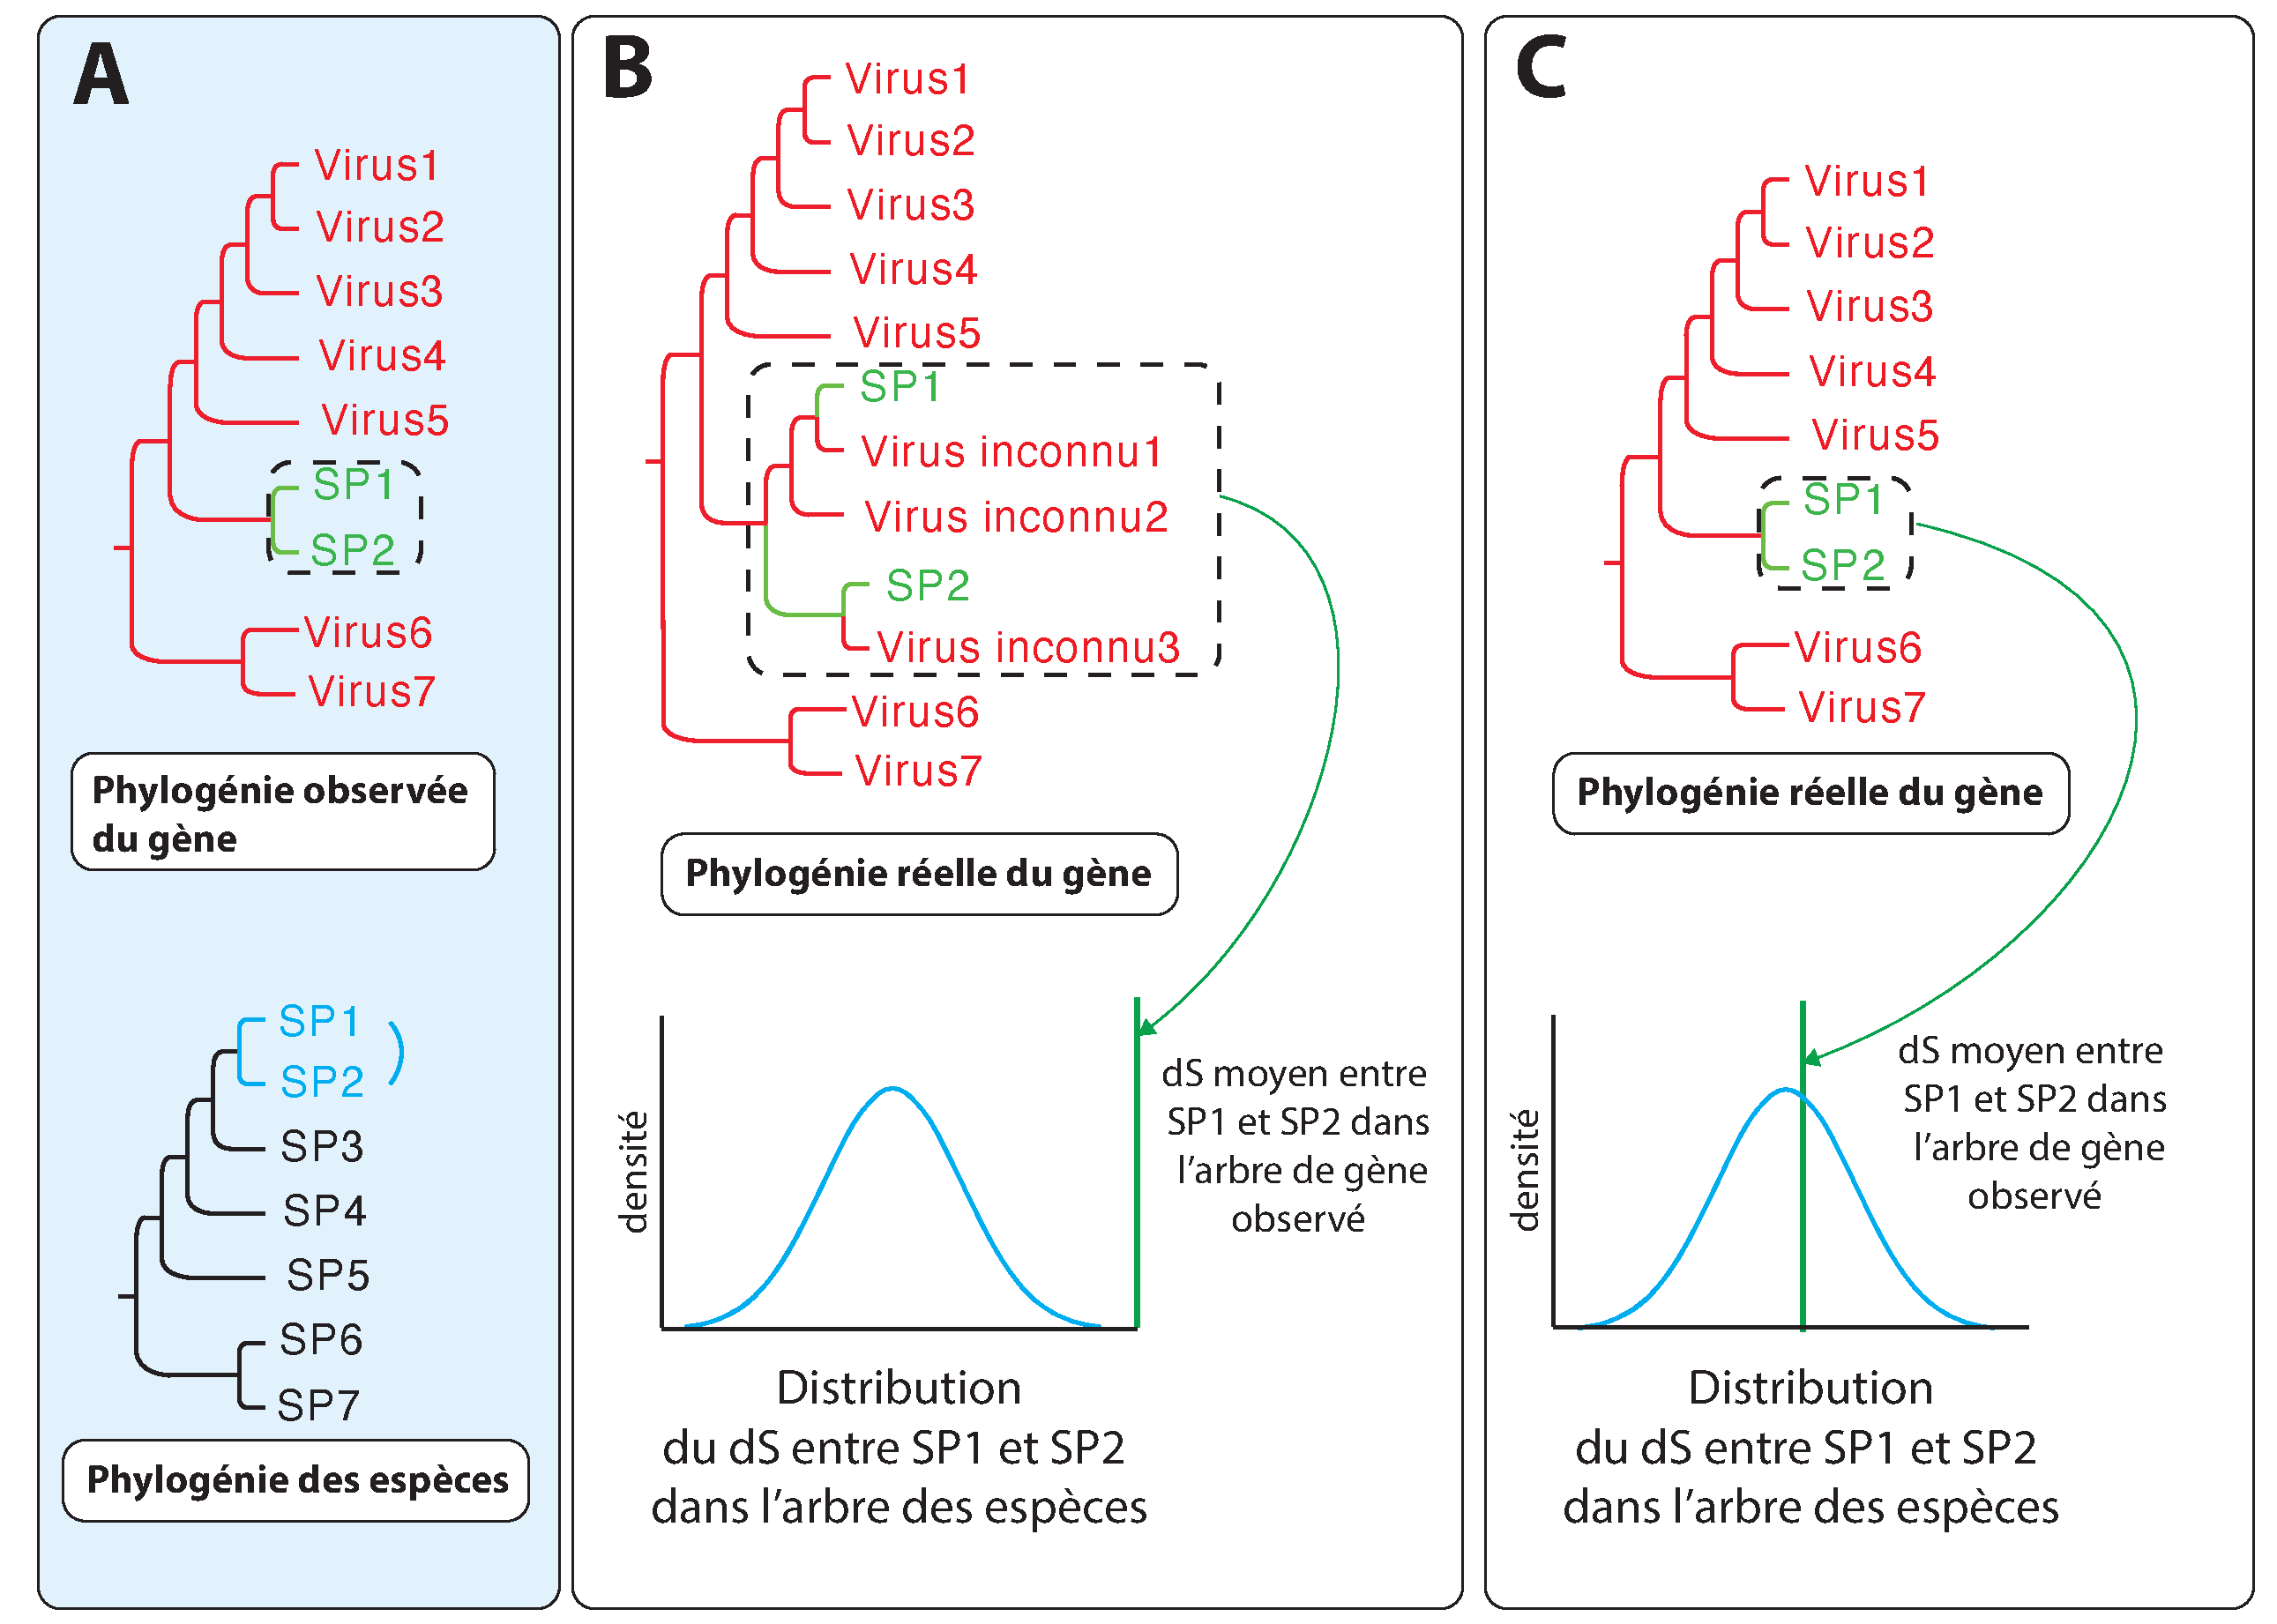
\includegraphics[width=\linewidth,height=\textheight,keepaspectratio]{PhD-master/figures/Biais_dNdS.pdf}
\caption[Methode:Exemple du biais de l'inférence de \textit{dN/dS} lorsqu'il manque des espèces dans l'arbre]{\textbf{Exemple du biais de l'inférence de \textit{dN/dS} lorsqu'il manque des espèces dans l'arbre}.}
\label{figure:Biais_dNdS}
\end{figure}

D'autres moyens existent pour étudier le caractère domestiqué d'un gène viral. Par exemple en étudiant de leur profil d'expression. Pour cela, lorsque des lectures RNAseq sont disponibles sur NCBI (RSA) pour l'espèce, nous les pouvons mapper ces reads le long des génomes assemblés. À l'aide de la couverture de ces reads, nous pouvons ainsi évaluer si un gène candidat est exprimé dans différents tissus ou non (\figurename{\ref{figure:Histoire_EVEs-domestication}}-7). Il faut néanmoins garder à l'esprit que certains papiers décrivent des profils d'expression d'EVEs n'ayant pourtant aucune fonction apparente dans les génomes. En effet, de telles observations pourraient être liées à une insertion récente d'un génome viral, expliquant une transcription encore intacte des EVEs \citep{cheng_brown_2014}. Enfin, une autre manière pouvant donner une idée de l'aspect fonctionnel des insertions peut être l'absence de codons stop prématurés ainsi qu'une longueur suffisamment grande des ORFs comparé à la longueur de l'ORF retrouvé chez l'espèce virale (\figurename{\ref{figure:Histoire_EVEs-domestication}}-8) (par exemple parmi les 39 EVEs retrouvés chez trois espèces de \textit{Leptopilina}, la longueur minimum correspondait à 95\% de la taille retrouvée chez l'ORF du virus le plus proche : LbFV) (Di Giovanni et al., 2020).

D'autres pistes inexplorées pendant ma thèse comme la prédiction de structures tridimensionnelles des protéines ou bien des indices de sélection traductionnelle pourraient également être adaptées et complémentaires pour inférer de la sélection vis-à-vis des copies de gènes viraux endogénisés.

Concernant les indices de sélection traductionnelle, en raison de la sélection traductionnelle, les gènes à haut niveau d'expression ont un biais de codon plus fort que les gènes à faible niveau d'expression \citep{hiraoka_codon_2009,zhou_non-optimal_2013}. Par conséquent, \cite{sharp_codon_1987} ont proposé l'indice d'adaptation des codons (CAI) pour mesurer le biais d'utilisation des codons synonymes pour une séquence de gènes testée en comparant la similarité entre l'utilisation des codons synonymes d'un gène et la fréquence des codons synonymes d'ensembles de gènes de référence hautement exprimés validés. Les valeurs de l'indice CAI sont comprises entre 0 et 1, les valeurs les plus élevées indiquant une plus grande similarité de l'utilisation des codons synonymes avec le niveau de référence/expression plus élevé \citep{puigbo_caical_2008}. 

La méthode impliquant la prédiction de structure tridimensionnelles peut nous permettre de savoir si les protéines codées par ces gènes d'origine virale dans les génomes eucaryotes peuvent se plier en structures tridimensionnelles (3D) raisonnables portant des fonctions moléculaires connues dans des bases de données. Ce type d'analyse peut par exemple être effectué en utilisant des programmes de prédiction de structure par apprentissage profond, AlphaFold2 \citep{jumper_highly_2021} ou bien RoseTTAFold \citep{baek_accurate_2021}. L'idée sous-jacente étant, à partir de ces modèles de protéines, d'évaluer leur niveau de fonctionnalité en les comparant avec une base de donnée connue, en utilisant par exemple le programme DeepFRI \citep{gligorijevic_structure-based_2021} pour l'évaluation fonctionnelle. Dans ce programme par exemple, une annotation de fonctions moléculaires des protéines virale se voit attribuer des scores de confiance fiables avec un seuil de signification associé. Si la protéine dépasse ce seuil, cela indique fortement que la protéine peut se replier sur une structure 3D correcte, reconnaissable et fonctionnelle.

Enfin, bien évidemment, l'utilisation de méthodes telles que l'ARN interférence ou bien des méthodes Crispr restent des méthodes de choix pour valider expérimentalement la fonction d’une protéine. Seulement, ces méthodes sont couteuses et inexploitables sur un grand nombre des gènes candidats. Elles doivent donc être utilisées sur des candidats spécifiques, comme cela a récemment été le cas dans une étude de transferts horizontaux de gènes entre des bactéries et des papillons. Dans cette étude, les chercheur.euses ont réussi à désactiver un gène transféré horizontalement depuis le génome d'une bactérie vers le génome de papillon et dont la fonction serait impliqué la cour des mâles chez les lépidoptères \cite{li_hgt_2022}.
